% \documentclass[12pt]{article}
\documentclass[12pt]{ctexart}
\usepackage[utf8]{inputenc}

\usepackage[english]{babel}
\usepackage[dvips]{epsfig}
\usepackage{amsmath}
\usepackage{amssymb}
\usepackage{amsfonts}
\usepackage{amsthm}
\usepackage{amsbsy}
\usepackage{amsgen}
\usepackage{amscd}
\usepackage{amsopn}
\usepackage{amstext}
\usepackage{amsxtra}
\usepackage{mathrsfs}
\usepackage{enumitem}
\usepackage{graphicx}
\usepackage{verbatim}
\usepackage{epstopdf}
\usepackage{float}
\usepackage[all,cmtip]{xy}
\usepackage{accents}
\usepackage{sseq}
\usepackage{url}
\usepackage{hyperref}
\usepackage{makeidx}
\usepackage{siunitx}
\usepackage{xcolor}
\usepackage{physics}

%%%%%%%%% 版面设置 %%%%%%%%%%%%%%%%%%%%%%%%%%%%%%%%%%%%%%
\usepackage{geometry}
\usepackage{titlesec}
\usepackage{fancyhdr}\pagestyle{empty}
\titleformat*{\section}{\large\bfseries}

%
\geometry{
	a4paper,
	total={170mm,240mm},
	left=20mm,
	top=30mm,
}

%Bitte nicht einstellen
\renewcommand{\figurename}{Abbildung}
\renewcommand{\tablename}{Tabelle}
\pagestyle{fancyplain}
\headheight 35pt
\lhead{\name}
\chead{\textbf{\Large \Title}}
\rhead{\due\\\today}
\lfoot{}
\cfoot{}
\rfoot{\small\thepage}
\headsep 1.5em

%%%%%%%%%%%%%%%%%%%%%%%%%%%%%%%%%%%%%%%%%%%%%%%%%%%%%%

\newtheorem{thm}{Theorem}[section]

% 定义解题环境
\theoremstyle{remark}
\newtheorem{remark}[thm]{Remark}
\newtheorem{theorem}{Theorem}
\newtheorem{observation}[thm]{Observation}

\theoremstyle{definition}
\newtheorem{problem}{\text{}}
\newtheorem{Problem}{\text{Problem}}
\newtheorem*{solution}{解}
\newtheorem*{Answer}{Answer}
\newtheorem{example}{Example} 

%%%%%%%%%%%%%%%%%%%%%%%%%%%%%%%%%%%%%%%%%%%%%%%%%%%%%%%%%%%%%%%%%%
\newcommand\name{陈景龙22120307}
\newcommand\due{-}
\newcommand{\emptyline}{\vspace{0.6\baselineskip}}
% \usepackage{enumerate}

\newcommand\Title{最优化方法笔记}
\renewcommand\due{due: 16 weeks}
\newtheorem*{theorem}{定理}


\begin{document}

总成绩=平时成绩(30\%)+ 小论文(20\%)+期末考试成绩(50\%)
\section{Introduction}
\begin{remark}
    给定二次型 $f(X) = X^T AX$,若对 $\forall X \neq 0$,都有 $f(X) = X^T AX > 0$ 成立,则称 $f(X)$ 为正定二次型,$A$ 为正定矩阵。

    对于 $n$ 阶实对称矩阵 $A$,下列命题等价:
    \begin{itemize}
        \item $A^T AX$ 是正定二次型(或 $A$ 是正定矩阵)
        \item $A$ 的 $n$ 个顺序主子式都大于 0
        \item $A$ 的 $n$ 个特征值都大于 0
        \item 存在可逆矩阵 $P$,使得 $A = P^T P$
    \end{itemize}
\end{remark}

\begin{remark}
    给定二次型 $f(X) = X^T AX$,若对 $\forall X \neq 0$,都有 $f(X) = X^T AX \ge 0$ 成立,则称 $f(X)$ 为半正定二次型,$A$ 为半正定矩阵。

    对于 $n$ 阶实对称矩阵 $A$,下列命题等价:
    \begin{itemize}
        \item $A^T AX$ 是半正定二次型(或 $A$ 是半正定矩阵)
        \item $A$ 的所有主子式都大于等于 0,而且至少有一个等于 0
        \item $A$ 的 $n$ 个特征值都大于等于 0,而且至少有一个等于 0
    \end{itemize}
\end{remark}

\begin{remark}
    设 $S \subseteq E^n$,若对 $\forall x, y \in S, \forall \lambda \in [0, 1]$,都有 $\lambda x + (1 - \lambda)y \in S$,则称 $S$ 为凸集。
    \begin{itemize}
        \item $x_1, \dots, x_k \in S, \lambda_1 + \cdots + \lambda_k = 1$,称 $\sum_{i = 1}^k \lambda_ix_i$ 为 $x_1, \dots, x_k$ 的凸组合
        \item $S$ 是非空凸集,$x\in S$,若由 $x = \lambda x_1 + (1 - \lambda)x_2$,其中 $\lambda \in (0, 1), x_1, x_2 \in S$,必推出 $x = x_1 = x_2$,则称 $x$ 是 $S$ 的极点。
        \item $S$ 是 $E^n$ 中的闭凸集,$d \in E^n, d \neq 0$,如果对 $\forall x \in S$,有 $\left\{x + \lambda d | \lambda > 0\right\} \subset S$,则称向量 $d$ 为 $S$ 的方向。若 $S$ 的方向 $d$ 不能表示为集合的两个不同方向的\textbf{正线性组合},则称 $d$ 为 $S$ 的极方向。
    \end{itemize}
\end{remark}

\begin{remark}
    设 $S = \left\{x | Ax = b, x \ge 0\right\}$ 为非空多面集,则有
    \begin{itemize}
        \item 极点集非空,且存在有限个极点
        \item 极方向集合为空集的充要条件是 $S$ 有界;若 $S$ 无界,则存在有限个极方向
        \item (多面集表示定理)$x \in S$ 的充要条件是 \begin{gather*}
            x = \sum_{j = 1}^k \lambda_j x^{(j)} + \sum_{j = 1}^l \mu_j d^{(j)}\\
            \lambda_j \ge 0, \forall j = 1, \dots, k\\
            \sum_{j = 1}^k \lambda_j = 1\\
            \mu_j \ge 0, \forall j = 1, \dots, l
        \end{gather*}
    \end{itemize}
\end{remark}

\begin{remark}
    凸集分离定理:
    \begin{itemize}
        \item 设 $S$ 为 $E^n$ 的闭凸集,$y\notin S$,则存在唯一的 $\overline{x} \in S$,使得\[ \|y - \overline{x}\| = \sideset{}{}{\operatorname{inf}}_{x \in S}\|y - x\| > 0 \]
        $\overline{x}$ 是这一最小距离点 $\Leftrightarrow (y - \overline{x})^T(\overline{x} - x) \ge 0, \forall x \in S$。

        \item 设 $S$ 是 $E^n$ 的非空闭凸集,$y\notin S$,则存在非零向量 $p$ 以及数 $\varepsilon > 0$,使得对 $\forall x \in S$,有 $p^T y \ge \varepsilon + p^T x$
        
        \item 设 $S$ 是 $E^n$ 的非空凸集,$y\in \partial S$,则存在非零向量 $p$,使得对 $\forall x \in clS$($S$ 的闭包,由 $S$ 的内点和边界点组成),有 $p^Ty \ge p^Tx$。
        
        \item 设 $S_1$ 和 $S_2$ 是 $E^n$ 的两个非空凸集,$S_1 \cap S_2 = \emptyset$,则存在非零向量,使得\[p^Ty \ge p^T x \quad \text{其中}\forall y \in S_1, \forall x \in S_2\]
    \end{itemize}
\end{remark}

\begin{remark}
    两个系统恰有一个有解:
    \begin{itemize}
        \item Farkas 引理:设 $A$ 为 $m\times n$ 矩阵,$c$ 为 $n$ 维列向量,则 $Ax \le 0, c^Tx > 0$ 有解的充分条件是 $A^Ty = c, y\ge 0$ 无解。
        \item Gordan定理:给定矩阵 $\boldsymbol{A} \in \mathbb{R}^{m\times n}$,下列两个系统只有一个有解
        \begin{gather*}
            \boldsymbol{A}x < 0\\
            \boldsymbol{y} \ge 0, \boldsymbol{y} \neq 0, \boldsymbol{A}^T\boldsymbol{y} = 0
        \end{gather*}
    \end{itemize}
\end{remark}

\begin{remark}
    设 $S$ 是 $E^n$ 中的非空凸集,$f(x)$ 是定义在 $S$ 上的实函数,如果对于每一对 $x_1, x_2 \in S$ 及每一个 $\lambda, 0\le \lambda \le 1$ 都有 \[f(\lambda x_1 + (1 - \lambda)x_2) \le \lambda f(x_1) + (1 - \lambda)f(x_2)\]
    则称函数 $f(x)$ 为 $S$ 上的凸函数。

    凸函数的根本重要性:设 $S$ 是 $E^n$ 中的非空凸集,$f$ 是定义在 $S$ 上的凸函数,则 $f$ 在 $S$ 上的局部极小点事整体极小点,且极小点的集合是凸集。
\end{remark}

\begin{remark}
    $f(x)$ 是凸集 $S$ 上的凸函数,对每一个实数 $c$,则集合 $S_c = \left\{x | x \in S, f(x) \le c\right\}$ 是凸集。
\end{remark}

\begin{remark}
    凸函数的判别:
    \begin{itemize}
        \item (一阶充要条件)设 $S$ 是 $E^n$ 中的非空开凸集,$f(x)$ 是定义在 $S$ 上的\textbf{可微}函数,则 $f(x)$ 为凸函数的充要条件是对任意两点 $x_1, x_2 \in S$,有 \[f(x_2) \ge f(x_1) + \nabla f(x_1)^T(x_2 - x_1)\]
        $f(x)$ 为严格凸函数的充要条件是对任意互不相同两点 $x_1, x_2 \in S$,有 \[f(x_2) > f(x_1) + \nabla f(x_1)^T(x_2 - x_1)\]

        几何意义:$f(x)$ 是凸函数当且仅当任意点处的切线增量不超过函数的增量。
        \item (二阶充要条件)设 $S$ 是 $E^n$ 中的非空开凸集,$f(x)$ 是定义在 $S$ 上的\textbf{二次可微}函数,则 $f(x)$ 为凸函数的充要条件是对任意 $x \in S$,$f(x)$ 在 $x$ 处的Hessian矩阵 $\nabla ^2f(x)$ 是半正定的。
        
        $f(x)$ 为严格凸函数的充要条件是对任意 $x \in S$,$f(x)$ 在 $x$ 处的Hessian矩阵 $\nabla ^2f(x)$ 是正定的。
    \end{itemize}
\end{remark}

\begin{remark}
    设 $f(x)$ 是定义在凸集 $S$ 上的可微凸函数,若 $\exists x^* \in S$,使对 $\forall x \in S$,都有 \[\nabla f(x^*)^T(x - x^*) \ge 0\]
    则 $x^*$ 是 $f(x)$ 在凸集 $S$ 上的全局极小点。
\end{remark}

\begin{remark}
    凸规划:求凸函数在凸集上的极小点。
    \begin{align*}
        \min \quad &f(x)\\ 
        s.t. \quad &g_{i}(x) \le 0, i=1, \cdots, m \\  
        &h_{j}(x)=0, j=1, \cdots, l 
    \end{align*}
    若 $f(x)$ 是凸函数,$g_i(x)$ 是凸函数,$h_j(x)$ 是线性函数,则原问题为凸规划。
    \begin{itemize} 
        \item 凸规划的局部极小点就是整体极小点
        \item 且极小点的集合为凸集
    \end{itemize}
\end{remark}

\section{LP 基本性质}
\begin{remark}
    LP 基本定理:
    \begin{itemize}
        \item 可行域的极点对应 LP 问题的基本可行解
        \item LP 的最优解一定可以在基本可行解中找到
        \item 设 $S$ 是 LP 的可行域,$\bar{x} \in S$,则 $\bar{x}$ 是 $S$ 的极点 $\Longleftrightarrow \bar{x}$ 是 LP 的基本可行解
        \item 如果LP有可行解,则一定存在基本可行解
        \item 如果LP有最优解,则存在一个基本可行解是最优解
        \item 若LP问题有最优解,则要么最优解唯一,要么有无
        穷多最优解
    \end{itemize}
\end{remark}

\section{单纯形法}
\begin{remark}
    最优解一定在极点达到,而极点对应于基本可行解,求解线性规划问题归结为找最优基本可行解。可以从一个基本可行解出发,求一个使目标丽数值有所改善的基本可行解:通过不断改进基本可行解,力图达到最优基本可行解。
\end{remark}

\begin{remark}
    \[(L P)\left\{\begin{array}{lc}
        \min & f(x)=c x \\
        \text { s.t. } & A x=b \\
        & x \geq 0
    \end{array}\right.\]
    其中 $A$ 是 $m \times n$ 矩阵,秩为 $m$,$c$ 是 $n$ 维列向量,$b\ge 0$ 是 $m$ 维列向量。
    \begin{itemize}
        \item 初始基本可行解
            $A = (P_1, \dots, P_m, P_{m + 1}, \dots, P_n) = \begin{pmatrix}
                B & N
            \end{pmatrix}$

            基本解 $x^{(0)} = \begin{pmatrix}
                B^{-1}b \\
                0
            \end{pmatrix}$,若 $B^{-1}b \ge 0$,则 $x^{(0)}$ 是基本可行解。

            目标函数 $f_0 = cx^{(0)} = \begin{pmatrix}
                C_B & C_N
            \end{pmatrix} \begin{pmatrix}
                B^{-1}b \\
                0
            \end{pmatrix} = C_BB^{-1}b$
        \item 从初始基本可行解出发,求一个改进的基本可行解。
        \item 进基和终止条件
            \[x=\left(\begin{array}{l}
                x_{B} \\
                x_{N}
                \end{array}\right),A x=b \Rightarrow\begin{pmatrix}
                    B & N
                \end{pmatrix}\left(\begin{array}{l}
                x_{B} \\
                x_{N}
                \end{array}\right)=B x_{B}+N x_{N}=b \Rightarrow x_{B}=B^{-1}b-B^{-1} N x_{N}\]
            目标函数值
            \begin{align*}
                f = cx &= \begin{pmatrix}
                    c_B & c_N
                \end{pmatrix}\begin{pmatrix}
                    x_B \\
                    x_N
                \end{pmatrix} = c_Bx_B + c_Nx_N \\
                &= c_B(B^{-1}b - B^{-1}Nx_N) + c_Nx_N \\
                &= c_BB^{-1}b - (c_BB^{-1}N - c_N)x_N \\
                &= f_0 - \sum_{j\in R}(c_BB^{-1}P_j - c_j)x_j \quad R :\text{非基变量下标集} \\
                &=f_0 - \sum_{j\in R}(z_j - c_j)x_j
            \end{align*}
            \begin{enumerate}
                \item 如果 $\forall j\in R$,有 $z_j - c_j \le 0$,则 $x^{(0)}$ 为最优解;
                \item 否则 $z_k - c_k = \max_{j \in R}\left\{z_j - c_j\right\}$,$P_k$ 为进基向量,$x_k$ 为进基变量,$x_k = 0 \to x_k > 0$。
            \end{enumerate}
        \item 出基下标和进基变量的值
        
            $Ax = b$ 解的变化,原 $x_B = B^{-1}b - B^{-1}Nx_N$,$x_k$ 由 0 变为正以后,$x_B = B^{-1}b - B^{-1}P_kx_k$,$x_B = \bar{b}-y_{k} x_{k}$,其中 $\bar{b} = B^{-1}b,y_k = B^{-1}P_k$。
            \begin{enumerate}
                \item 若 $y_{ik}\le 0$,则 $\forall x_k \Longrightarrow x_{B_i} > 0,x_k$ 可以取无限大,故 $f\to -\infty$,原问题无界。
                \item 要满足 $x_B = \bar{b}-y_{k} x_{k} \ge 0$,则取 $x_k = \min(\frac{\bar{b}}{y_{ik}},y_{ik}>0) = \frac{\bar{b}}{y_{rk}} > 0$,$r$ 为出基下标。
            \end{enumerate}
    \end{itemize}
\end{remark}

\begin{remark}
    单纯形表
    \begin{itemize}
        \item 做初等行变换
        \item 若 $z_j - c_j > 0$,对应的系数列向量 $\le 0$,则该 LP 存在无界解;
        \item 若某个非基变量的检验数为 0,则该 LP 存在多个最优解。
    \end{itemize}
    \begin{figure}[htbp]
        \centering
        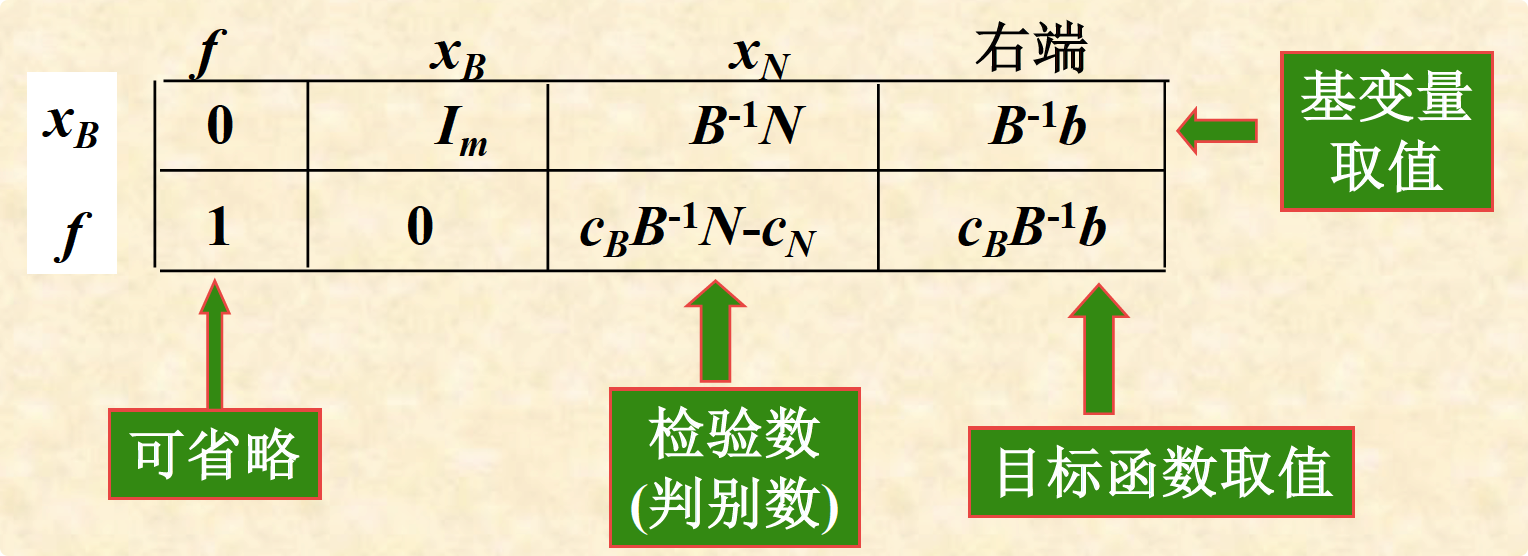
\includegraphics[width=0.8\textwidth]{./figures/img1.png}
        \caption{单纯形表 \label{fig1}}
    \end{figure}
\end{remark}

\section{对偶理论}
\begin{remark}
    对称形式的对偶规划的要点
    \begin{itemize}
        \item min变成max,价值系数 $c$ 与右端向量 $b$ 互换,系数矩阵 $A$ 转置,$\ge$ 变为 $\le$
        \item 原问题中约束条件的个数 = 对偶问题中变量的个数
        \item 原问题中变量的个数 = 对偶问题中约束条件的个数
        \item $\begin{cases}
            \min \quad &c^Tx\\
            s.t. \quad &Ax \ge b\\
            & x \ge 0
        \end{cases}\quad  \Longrightarrow \quad \begin{cases}
            \max\quad &b^Tw \\
            s.t.\quad &A^Tw \le c\\
            &w \ge 0
        \end{cases}$
        \item 对偶问题的对偶问题是原问题
        \item 一般情形 LP 问题的对偶问题\[\begin{cases}
            \min \quad & c^Tx\\
            s.t. \quad & A_1x \ge b_1\\
            & A_2x = b_2\\
            &A_3x \le b_3\\
            &x \ge 0
        \end{cases} \quad \Longrightarrow \quad \begin{cases}
            \max \quad & b_1^Tw_1 + b_2^Tw_2 + b_3^Tw_3\\
            s.t. \quad & A_1^Tw_1 + A_2^Tw_2 + A_3^Tw_3 \le c\\
            &w_1 \ge 0, w_2\  \text{free}, w_3 \le 0
        \end{cases}\]
        图\ref{fig2}中,右边是原问题,左边是对偶问题。
        \begin{figure}[htbp]
            \centering
            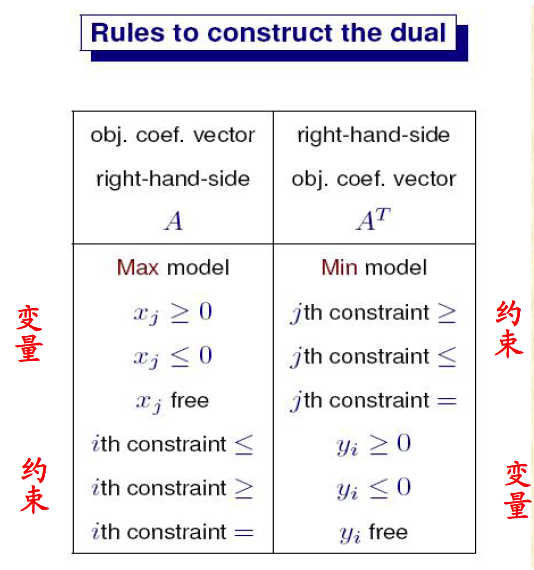
\includegraphics[width=0.4\textwidth]{./figures/img2.png}
            \caption{LP问题的对偶问题转换规则 \label{fig2}}
        \end{figure}
        \[\begin{cases}
            \min \quad & 2x_1 + x_2 + 2x_3\\
            s.t. \quad & x_1 + x_2 + 2x_3 \ge 1\\
            &x_1 - x_2 + x_3 \le 2\\
            &-x_1 + x_2 + x_3 = 1\\
            &x_1 \ge 0, x_2 \ \text{free}, x_3 \le 0
        \end{cases} \Longrightarrow \begin{cases}
            \max \quad & w_1 + 2w_2 + w_3\\
            s.t. \quad & w_1 + w_2 - w_3 \le 2\\
            &w_1 - w_2 + w_3 = 1\\
            &2w_1 + w_2 + w_3 \ge 2\\
            &w_1 \ge 0, w_2 \le 0, w_3 \ \text{free}
        \end{cases}\]
        原问题的变量对应对偶问题的约束,并且\textbf{符号改变}。
    \end{itemize}
\end{remark}

\begin{remark}
    对偶问题的基本性质
    \begin{itemize}
        \item 弱对偶定理:若 $x^{(0)}, w^{(0)}$ 分别是原问题(P)和对偶问题(D)的可行解,则 $c^Tx^{(0)} \ge b^Tw^{(0)}$,即最小化目标的函数值大于等于最大化目标的函数值。\begin{itemize}
            \item Proof:\begin{itemize}
                \item $Ax^{(0)} \ge b, x^{(0)} \ge 0$,同时 $A^Tw^{(0)} \le c, w^{(0)} \ge 0$,故 $c^Tx^{(0)} \ge (A^Tw^{(0)})^Tx^{(0)} = (w^{(0)})^TAx^{(0)} \ge (w^{(0)})^Tb = b^Tw^{(0)}$
            \end{itemize}
            \item 推论1:若原问题(P)或对偶问题(D)有无界解,则其对偶问题(D)或原问题(P)无可行解
            \item 推论2:极大化问题的任何一个可行解所对应的目标函数值都是其对偶问题的目标函数值的下界。
            \item 推论3:极小化问题的任何一个可行解所对应的目标函数值都是其对偶问题的目标函数值的上界。
        \end{itemize}
        \item 最优性准则:若 $x^{(0)}, w^{(0)}$ 分别为原问题(P)对偶问题(D)的可行解,且 $cx^{(0)} = w^{(0)}b$,则 $x^{(0)}, w^{(0)}$ 分别为原问题(P)对偶问题(D)的最优解
        \item 强对偶定理:若原问题(P)和对偶问题(D)均有可行解,则原问题(P)和对偶问题(D)均有最优解,且(P)(D)的最优目标函数值相等。\begin{itemize}
            \item 推论:若问题(P)或(D)无可行解,则其对偶问题(D)或(P)或者无可行解,或者目标函数值趋于无穷。
            \item 推论:在用单纯形法求解LP问题(P)的最优单纯形表中松弛变量的检验数的相反数为单纯形乘子$w = c_BB^{-1}$,也就是其对偶问题(D)的最优解.
        \end{itemize}
    \end{itemize}
\end{remark}

\begin{remark}
    总结:
    \begin{itemize}
        \item 原问题有最优解,对偶问题一定有最优解,且相同
        \item 原问题有无界解,则对偶问题无可行解
        \item 原问题无可行解,则对偶问题有无界解或无可行解
    \end{itemize}
\end{remark}

\begin{remark}
    互补松弛定理:设 $x^{(0)}, w^{(0)}$ 分别是 (P), (D) 问题的可行解,则 $x^{(0)},w^{(0)}$ 分别为 (P), (D) 的最优解的充要条件是 $\forall i, j (1 \le i \le m, 1\le j \le n)$ 有 \begin{itemize}
        \item 若 $x_j^{(0)} > 0$,则 $w^{(0)}P_j = c_j$
        \item 若 $w^{(0)}P_j < c_j$,则 $x_j^{(0)} = 0$
        \item 若 $w_i^{(0)} > 0$,则 $A_ix^{(0)} = b_i$
        \item 若 $A_ix^{(0)} > b_i$,则 $w_i^{(0)} = 0$
    \end{itemize}
    即 $\begin{cases}
        (c - w^{(0)}A)x^{(0)} = 0\\
        w^{(0)}(Ax^{(0)} - b) = 0
    \end{cases}$,其中 $P_j$ 是 $A$ 的第 $j$ 列,$A_i$ 是 $A$ 的第 $i$ 行。

    互补松弛定理(非对称形式)

    设 $x^{(0)}$ 和 $w^{(0)}$ 分别是 $\begin{cases}
        \min \quad & c^Tx \\
        s.t. \quad & Ax = b\\
        &x \ge 0
    \end{cases}$ 和 $\begin{cases}
        \max \quad & b^Tw \\
        s.t. \quad & A^Tw \le c
    \end{cases}$ 的可行解,则 $x^{(0)}$ 和 $w^{(0)}$ 是最优解的充要条件是 $\forall j$ \begin{itemize}
        \item $x_j^{(0)} > 0 \Longrightarrow w^{(0)}P_j = c_j$
        \item $w^{(0)}P_j < c_j \Longrightarrow x_j^{(0)} = 0$
    \end{itemize}
\end{remark}

\begin{remark}
    对偶单纯形法步骤:
    \begin{enumerate}
        \item 化标准型,建立初始单纯形表
        \item 判断,若 $B^{-1}b \ge 0$,则已得到最优解
        \item 换基迭代 \begin{enumerate}
            \item 确定换出变量,$\bar{b_r} = \min_i\left\{\bar{b_i}\right\} < 0, x_r$ 为换出变量
            \item 确定换入变量,$\min_{j}\left\{\frac{z_j - c_j}{y_{rj}}\ |\ y_{rj} < 0\right\} = \frac{z_k - c_k}{y_{rk}}$,$x_k$ 为换入变量(若所有 $y_{rj} \ge 0$,则该 LP 问题无可行解)
            \item 换基迭代,$y_{rk}$ 为主元
        \end{enumerate}
        \item 回到第 2 步
    \end{enumerate}
\end{remark}

\begin{remark}
    对偶单纯形法与原单纯形法的区别:
    \begin{itemize}
        \item 原单纯形法保持原问题的可行性,对偶单纯形法保持所有检验数 $wP_j - c_j \le 0$,即保持对偶问题的可行性。
        \item 特点:先选择出基变量,再选择进基变量。
    \end{itemize}
\end{remark}


\section{算法概述}
\begin{remark}
    一类线搜索下降迭代算法的步骤:
    \begin{enumerate}
        \item 选定某一初始点 $x^{(0)}$,置 $k = 0$;
        \item 确定搜索方向 $d^{(k)}$;
        \item 从 $x^{(0)}$ 出发,沿方向 $d^{(k)}$ 求步长 $\lambda_k$,以产生下一个迭代点 $x^{(k + 1)}$;
        \item 检查 $x^{(k + 1)}$ 是否为极小点或近似极小点,若是,则停止迭代;否则,令 $k:= k + 1$,返回2。
    \end{enumerate}

    选取搜索方向是最关键的一步,各种算法的区别, 主要在于确定搜索方向的方法不同。
\end{remark}

\begin{remark}
    解集合:把满足某些条件的点集定义为解集合.当迭代点属于该集合时,停止迭代。
    
    常用的解集合:
    \begin{itemize}
        \item $\Omega = \left\{\bar{x}\ |\ \|\nabla f(\bar{x})\| = 0\right\}$
        \item $\Omega = \left\{\bar{x}\ |\ \bar{x} \text{为KKT点}\right\}$
        \item $\Omega = \left\{\bar{x}\ |\ \bar{x} \in S, f(\bar{x}) \le b\right\}$,其中 $b$ 是某个可接受的目标函数值。
    \end{itemize}
\end{remark}

\begin{remark}
    实用收敛准则
    \begin{itemize}
        \item $\|x^{(k + 1)} - x^{(k)}\| < \varepsilon$ 或者 $\frac{\|x^{(k + 1)} - x^{(k)}\|}{\|x^{(k)}\|} < \varepsilon$
        \item $f(x^{(k)}) - f(x^{(k + 1)}) < \varepsilon$ 或者 $\frac{f(x^{(k)}) - f(x^{(k + 1)})}{|f(x^{(k)})|} < \varepsilon$
        \item $\|\nabla f(x^{(k)})\| < \varepsilon$ (无约束最优化中)
    \end{itemize}
\end{remark}

\begin{remark}
    Q-收敛速率(Quotient)

    设序列 $\left\{\gamma^{(k)}\right\}$ 收敛于 $\gamma^*$,定义满足 \[\lim _{k \rightarrow+\infty} \frac{\left\|\gamma^{(k+1)}-\gamma *\right\|}{\left\|\gamma^{(k)}-\gamma *\right\|^{p}}=\beta<\infty\] 的非负数 $p$ 的上确界为序列 $\left\{\gamma^{(k)}\right\}$ 的收敛级。
    \begin{itemize}
        \item 若序列的收敛级为 $p$,则称序列是 $p$ 级收敛的。
        \item 若 $p = 1$ 且 $0 < \beta < 1$,则称序列是以收敛比 $\beta$ 线性收敛的。
        \item 若 $p > 1$,或者 $p = 1$ 且 $\beta = 0$,则称序列是超线性收敛的。
        \item 收敛级 $p$ 越大,序列收敛得越快;当收敛级 $p$ 相同时,收敛比 $\beta$ 越小,序列收敛得越快。
    \end{itemize}
\end{remark}

\begin{remark}
    R-收敛速率(Root):

    设点列 $\left\{x_k\right\}$ 收敛到 $x^*$。若存在 $\kappa>0, q \in(0,1)$ 使 $\|x_k - x^*\| \le \kappa q^k$,则称点列 $\left\{x_k\right\}$ R-线性收敛到 $x^*$;若存在 $\kappa > 0$ 和收敛到 $0$ 的正数列 $\left\{q_k\right\}$ 使 $\|x_k - x^*\| \le \kappa \prod_{i = 1}^k q_i$,则称点列 $\left\{x_k\right\}$ R-超线性收敛到 $x^*$。

    \begin{itemize}
        \item Q-(超)线性收敛 $\Longrightarrow$ R-(超)线性收敛
    \end{itemize}
\end{remark}

\begin{remark}
    算法的二次终止性:若某个算法对任意的\textbf{正定二次函数},从任意的初始点出发,都能经有限步迭代达到其极小点,则称该算法具有二次终止性。
    
    用二次终止性作为判断算法优劣的原因:
    \begin{enumerate}
        \item 正定二次函数具有某些较好的性质,因此一个好的算法应能够在有限步内达到其极小点。
        \item 对于一般的目标函数,若在其极小点处Hesse矩阵正定\[f(x) =f\left(x^{*}\right)+\nabla f\left(x^{*}\right)^{T}\left(x-x^{*}\right) 
        +\frac{1}{2}(x-x *)^{T} \nabla^{2} f\left(x^{*}\right)\left(x-x^{*}\right)+o\left(\left\|x-x^{*}\right\|\right)\]
        因此可以猜想,对正定二次函数好的算法,对于一般目标函数也应具有较好的性质。
    \end{enumerate}
\end{remark}

\begin{remark}
    单纯形算法的复杂度为指数时间复杂度。
\end{remark}

\begin{remark}
    对于线性规划问题 \[\min_{\lambda \ge 0} \quad f(x^{(k)} + \lambda d^{(k)})\] 如果求得的 $\lambda_k$,使得 \[f(x^{(k)} + \lambda_kd^{(k)}) = \min_\lambda f(x^{(k)} + \lambda d^{(k)})\]则称该一维搜索为精确一维搜索,$\lambda_k$ 为最优步长。否则,该一维搜索为非精确一维搜索。
\end{remark}

\begin{remark}
    一维搜索\begin{itemize}
        \item 精确线搜索\begin{itemize}
            \item 试探法:黄金分割法、Fibonacci法、二分法
            \item 函数逼近法:Newton法、割线法、抛物线法、三次插值法
        \end{itemize}
        \item 非精确线搜索:Armijo 步长规则、Goldstein 步长规则、Wolfe步长规则
    \end{itemize}
\end{remark}

\begin{remark}
    函数逼近法:牛顿法

    基本思想:在极小点附近用二阶 Taylor 多项式近似。 \[\min \quad f(x)\]
    令 $\varphi(x)=f\left(x^{(k)}\right)+f^{\prime}\left(x^{(k)}\right)\left(x-x^{(k)}\right)+\frac{1}{2} f^{\prime \prime}\left(x^{(k)}\right)\left(x-x^{(k)}\right)^{2}$,又令 $\varphi^{\prime}(x)=f^{\prime}\left(x^{(k)}\right)+f^{\prime \prime}\left(x^{(k)}\right)\left(x-x^{(k)}\right)=0$,得 $\varphi(x)$ 的驻点,记 $x^{(k + 1)}$,则 $x^{(k+1)}=x^{(k)}-\frac{f^{\prime}\left(x^{(k)}\right)}{f^{\prime \prime}\left(x^{(k)}\right)}$。

    \begin{theorem}
        设 $f(x)$ 存在连续三阶导数,$\bar{x}$ 满足 $f^\prime(\bar{x}) = 0$,$f^{\prime\prime}(\bar{x}) \neq 0$,初点 $x^{(1)}$ 充分接近 $\bar{x}$,则牛顿法产生的序列 $\left\{x^{(k)}\right\}$ 至少以二级收敛速度收敛于 $\bar{x}$。
    \end{theorem}

    算法步骤:\begin{enumerate}
        \item 给定初始点 $x^{(0)}$,允许误差 $\varepsilon > 0$,置 $k = 0$。
        \item 若 $|f^\prime(x^{(k)})| < \varepsilon$,则停止计算,得点 $x^{(k)}$;否则转 3
        \item 计算点 $x^{(k + 1)} = x^{(k)} - \frac{f^\prime(x^{(k)})}{f^{\prime\prime}(x^{(k)}}$,置 $k = k + 1$,返回 2
    \end{enumerate}

    缺点:初始点选择十分重要。如果初始点靠近极小点,则可能很快收敛;如果初始点远离极小点,迭代产生的点列可能不收敛于极小点。
\end{remark}

\begin{remark}
    非精确搜索:
    \begin{itemize}
        \item Armijo 步长规则\begin{itemize}
            \item 设 $\beta > 0, \gamma \in (0, 1), \sigma \in (0, 1)$。取步长 $\lambda_k = \beta \gamma^{m_k}$,其中 $m_k$ 是满足下式的最小非负整数:\[f\left(x^{(k)}+\beta \gamma^{m} d^{(k)}\right) \leq f\left(x^{(k)}\right)+\sigma \beta \gamma^{m} \nabla f\left(x^{(k)}\right)^{T} d^{(k)}\]
            \item 根据目标函数的 Taylor 展开式,满足这种规则的步长一定存在。
        \end{itemize}
        \item Goldstein 步长规则\begin{itemize}
            \item 设 $\sigma \in (0, \frac{1}{2})$。取步长满足下式\begin{gather*}
                f\left(x^{(k)}+\lambda d^{(k)}\right) \leq f\left(x^{(k)}\right)+\sigma \lambda \nabla f\left(x^{(k)}\right)^{T} d^{(k)} \\
                f\left(x^{(k)}+\lambda d^{(k)}\right)>f\left(x^{(k)}\right)+(1-\sigma) \lambda \nabla f\left(x^{(k)}\right)^{T} d^{(k)}
            \end{gather*}
            \item 由于 $\lambda > 0$ 充分小时,第二式必不成立,故改规则在保证目标函数下降的前提下,使下一迭代点尽可能远离当前迭代点。
        \end{itemize}
        \item Wolfe 步长规则\begin{itemize}
            \item 设 $0 < \sigma_1 < \sigma_2 < 1$。取步长 $\lambda_k$ 满足下式\begin{gather*}
                f\left(x^{(k)}+\lambda d^{(k)}\right) \leq f\left(x^{(k)}\right)+\sigma_{1} \lambda \nabla f\left(x^{(k)}\right)^{T} d^{(k)} \\
                \nabla f\left(x^{(k)}+\lambda d^{(k)}\right)^{T} d^{(k)} \geq \sigma_{2} \nabla f\left(x^{(k)}\right)^{T} d^{(k)}
            \end{gather*}
            \item 该规则使函数 $f(x^{(k)} + \lambda d^{(k)})$ 的陡度在 $\lambda_k$ 点比在 $\lambda = 0$ 点有所减缓,从而使下一迭代点尽可能远离当前迭代点。
        \end{itemize}
    \end{itemize}
\end{remark}

\section{非线性规划的最优性条件}
\begin{remark}
    最优性条件 
    \begin{itemize}
        \item 设 $f(x)$ 为目标函数,$S$ 为可行域,$x^{(0)} \in S$, 若对 $\forall x \in S$,有 $f(x) \ge f(x^{(0)})$,则 $x^{(0)}$ 称为极小化问题 $\min f(x)$,$x \in S$ 的(全局)最优解。
        \item 设 $f(x)$ 为目标函数,$S$ 为可行域,若存在 $x^{(0)}$ 的 $S$ 邻域 \[N_{\varepsilon}\left(x^{0}\right)=\left\{x \mid\left\|x-x^{0}\right\|<\varepsilon, \varepsilon>0\right\}\]使得对 $\forall x \in S \cap N_\varepsilon(x^{(0)})$,有 $f(x) \ge f(x^{(0)})$,则 $x^{(0)}$ 称为极小化问题 $\min f(x)$,$x \in S$ 的局部最优解。
    \end{itemize}
\end{remark}

\begin{remark}
    无约束优化问题的最优性条件\[\min f(x) \quad \text{s.t. } x \in E^n\]
    \begin{itemize}
        \item 定义:对$\min f(x)$,设 $\bar{x} \in E^n$ 是任给一点,$d\neq 0$ ,若存在 $\delta > 0$,使得对任意的 $\lambda \in (0, \delta)$,有 $f(\bar{x} + \lambda d) < f(\bar{x})$,则称 $d$ 为 $f(x)$ 在点 $\bar{x}$ 处的下降方向。
        \item 引理:设函数 $f(x)$ 在点 $\bar{x}$ 可微,若存在 $d \neq 0$ 使 $\nabla f(\bar{x})^td < 0$,则存在 $\delta > 0$,使对 $\forall \lambda\in (0, \delta)$,有 $f(\bar{x} + \lambda d) < f(\bar{x})$
    \end{itemize}
\end{remark}

\begin{remark}
    无约束优化问题的最优性条件\begin{itemize}
        \item 一阶必要条件:设函数 $f(x)$ 在点 $\bar{x}$ 处可微,若 $\bar{x}$ 是局部极小点,则 $\nabla f(\bar{x}) = 0$
        \item 二阶必要条件:设 $f(x)$ 在 $\bar{x}$ 处二阶可微,若 $\bar{x}$ 是局部极小点,则 $\nabla f(\bar{x}) = 0$,且 Hessian 矩阵 $\nabla^2f(\bar{x})$ 是半正定的
        \item 充分条件:设函数 $f(x)$ 在点 $\bar{x}$ 处二次可微,若梯度 $\nabla f(\bar{x}) = 0$ ,且 Hessian矩阵 $\nabla^2f(\bar{x})$ 正定,则 $\bar{x}$ 是严格局部极小点。
        \item 设函数 $f(x)$ 在点 $\bar{x}$ 的邻域内二次可微,若梯度 $\nabla f(\bar{x}) = 0$,且Hessian矩阵 $\nabla^2f(x)$ \textbf{在该邻域内}半正定,则 $\bar{x}$ 是局部极小点。特别地,对于邻域内的任意点 $x\neq \bar{x}$,若 $\nabla^2f(x)$ 是正定矩阵,则 $\bar{x}$ 是一个严格的局部极小点。
        \item 设 $f(x)$ 是定义在 $E^n$ 上的可微凸函数,$\bar{x} \in E^n$,则 $\bar{x}$ 为整体极小点的充要条件是 $\nabla f(\bar{x}) = 0$.
    \end{itemize}
\end{remark}

\begin{remark}
    \text{}\begin{itemize}
        \item 定义:若 $f(x)$ 在点 $x^*$ 可微,并且 $\nabla f(x^*) = 0$。则 $x^*$ 称为 $f(x)$ 的一个驻点(平稳点),既不是极小点,也不是极大点的驻点称为鞍点。
    \end{itemize}
\end{remark}

\begin{remark}
    约束优化问题的最优性条件
    \begin{itemize}
        \item 定义:对$\underset{x \in E^n}{\min}f(x)$,设 $\bar{x} \in E^n$ 是任给一点,$d\neq 0$,若存在 $\delta > 0$,使得对任意的 $\lambda \in (0, \delta)$ 有 $f(\bar{x} + \lambda d) < f(\bar{x})$,则称 $d$ 为 $f(x)$ 在点 $\bar{x}$ 处的下降方向。\[F_0 = \left\{d\ |\ \nabla f(\bar{x})^td < 0\right\}\]称为点 $\bar{x}$ 处的下降方向集。
        \item 定义:设集合 $S \subset E^n$,$\bar{x} \in clS$,$d$ 为非零向量,若存在数 $\delta > 0$,使得对任意 $\lambda \in (0, \delta)$,都有 $\bar{x} + \lambda d \in S$ 则称 $d$ 为集合 $S$ 在 $\bar{x}$ 的可行方向。$D=\{d \mid d \neq 0, \bar{x} \in c l S, \exists \delta>0, \forall \lambda \in(0, \delta), \bar{x}+\lambda d \in S\}$ 是 $\bar{x}$ 处的可行方向锥。
        \item 几何最优性条件:考虑问题\[\min f(x), \quad \text{s.t. } x \in S\]设 $S$ 是 $E^n$ 的非空集合,$\bar{x} \in S$,$f(x)$ 在 $\bar{x}$ 处可微,若 $\bar{x}$ 是局部最优解,则 $F_0\cap D = \emptyset$
        \item 对于不等式约束优化问题\[\begin{cases}
            \min \quad &f(x)\\
            \text{s.t.} \quad &g_i(x) \ge 0, \quad i = 1, \dots, m
        \end{cases}\]
        可行域 $S = \left\{x\ |\ g_i(x) \ge 0, i = 1, \dots, m\right\}$
        \begin{itemize}
            \item 定义:若一个可行点 $\bar{x}$($\bar{x} \in S$ )使某个不等式约束$g_i(x) \ge 0$变成等式,即 $g_i(\bar{x}) = 0$,则该不等式约束称为关于可行点 $\bar{x}$ 的起作用约束(或等式约束);否则,若 $\bar{x}$ 使得某个 $g_i(\bar{x}) > 0$,则该不等式约束称为关于可行点 $\bar{x}$ 的不起作用约束(或松约束)。记 $I = \left\{i\ |\ g_i(\bar{x}) = 0, \bar{x} \in S\right\}$
            \item $G_0 = \left\{d \ |\ \nabla g_i(\bar{x})^td > 0, i \in I\right\}$ 称为 $S$ 在点 $\bar{x}$ 处的局部约束方向锥(或内方向锥)
            \item 设 $\bar{x} \in S$,$f(x)$ 和 $g_i(x)(i \in I)$ 在 $\bar{x}$ 处可微,$g_i(x)(i \notin I)$ 在 $\bar{x}$ 处连续,如果 $\bar{x}$ 是局部最优解,则 $F_0\cap G_0 = \emptyset$。
            \item Fritz John 条件:设 $\bar{x} \in S$, $f(x), g_i(x)(i \in I)$ 在 $\bar{x}$ 处可微,$g_i(x)(i\notin I)$ 在 $\bar{x}$ 处连续,若 $\bar{x}$ 是局部最优解,则存在不全为零的数 $w_0, w_i(i \in I)$,使得 \[\begin{cases}
                w_{0} \nabla f(\bar{x})-\sum_{i \in I} w_{i} \nabla g_{i}(\bar{x})=0 \\
                w_{0}, \quad w_{i} \geq 0, \quad i \in I
            \end{cases}\] $\bar{x}$ 称为 Fritz John 点,即满足Fritz John条件的点.
            \item KKT 条件:设 $\bar{x} \in S$, $f(x), g_i(x)(i \in I)$ 在 $\bar{x}$ 处可微,$g_i(x)(i\notin I)$ 在 $\bar{x}$ 处连续,若 $\bar{x}$ 是局部最优解,存在非负数 $w_i, i \in I$,使得\[\nabla f(\bar{x}) - \sum_{i \in I}w_i\nabla g_i(\bar{x}) = 0\]
            \item 设 $\bar{x} \in S, f, g_i$ 在 $\bar{x}$ 可微,$\left\{\nabla g_i(\bar{x}) | i \in I\right\}$;线性无关,若 $\bar{x}$ 是局部最优解,则存在数 $w_i, i=1, 2, \dots, m$,使得\[\begin{array}{l}
                \nabla f(\bar{x})-\sum_{\mathrm{i}=1}^{m} w_{i} \nabla g_{i}(\bar{x})=0 \\
                w_{i} g_{i}(\bar{x})=0 \quad i=1,2, \cdots, m \\
                w_{i} \geq 0 \quad i=1,2, \cdots, m 
            \end{array}\]
        \end{itemize}
    \end{itemize}
\end{remark}

\end{document}